\chapter{Komponenty systemu}
	Aby uruchomić system, nie wystarczy uruchomić Gazebo z modelami, należy zadbać także o odpowiednie przekazywanie informacji pomiędzy pakietami.
	Należy także przetestować modele, czy zachowują się poprawnie w prostych scenariuszach testowych, tak samo, jak testować się będzie program sterujący.
	Do tego potrzebne są programy wspomagające, które łączy się w różne konfiguracje, w zależności od scenariusza testowego.
	
	\begin{table}
		\centering
		\begin{tabular}{l r}
			Typ & Opis \\
			\hline
			\texttt{omnivelma\_msgs/Encoders} & Prędkości i pozycje kół z enkodera. \\
			\texttt{omnivelma\_msgs/Vels} & Prędkości kół. \\
			\texttt{omnivelma\_msgs/SetFriction} & Nadanie tarcia elementowi modelu. \\
			\texttt{omnivelma\_msgs/SetInertia} & Nadanie mas i momentu bezwładności obiektowi. \\
			\texttt{geometry\_msgs/Pose} & Pozycja i rotacja obiektu w przestrzeni kartezjańskiej. \\
			\texttt{geometry\_msgs/Twist} & Prędkość względna jakiegoś obiektu. \\
			\texttt{sensor\_msgs/LaserScan} & Jedno skanowanie LiDARa, wraz z nagłówkiem. \\
			\texttt{omnivelma\_msgs/Relative} & Odległość i kąt pomiędzy obiektami. \\
		\end{tabular}
		\caption{Typy i opisy wiadomości przekazywanych pomiędzy komponentami.}
		\label{tab:messages}
	\end{table}
	
	Niektóre typy mają dopisek \texttt{Stamped}, co oznacza że zawierają także nagłówek.
	Nagłówek posiada trzy pola:
	\begin{itemize}
		\item Numer sekwencyjny, zwiększany przez program wysyłający za każdym pakietem.
		\item Czas nadania pakietu, z dokładnością do nanosekund.
		\item Identyfikator ramki, według której podano dane, ramki zostały opisane dokładniej w \ref{sec:frames}.
	\end{itemize}
	
	Komponenty można podzielić na trzy typy:
	\begin{itemize}
		\item Generujące pakiety danych.
		\item Przekazujące i modyfikujące pakiety danych.
		\item Zbierające pakiety danych.
	\end{itemize}
	Poniżej każdy pakiet opisany jest bardziej szczegółowo, ten dokument nie ma za zadanie być programistyczną dokumentacją komponentów, dlatego 
	nie zagłębia się w dokładne składy przekazywanych struktur i ich nazwy.
	
	\section{Manualne sterowanie}
		To zaawansowany program do manualnego generowania zadanych prędkości, lub kierunku platformy.
		Ponieważ jest niezależny od reszty systemu, może być użyty do sterowania rzeczywistym robotem.
		Pozwala także na wyświetlanie aktualnych prędkości kół, generowanych przez enkodery.
		Ma nazwę kodową \texttt{lalkarz}, ponieważ steruje platformą, tak jak aktor steruje marionetką.
		
		\subsection{Program}
			Ten komponent jest plikiem wykonywalnym, skompilowanym ze źródeł w C++.
			Wykorzystując bibliotekę graficzną SFML, generuje okno z powierzchnią do rysowania na nim za pomocą OpenGL.
			Biblioteka ta pozwala również na bezproblemowe przechwytywanie zdarzeń z klawiatury, takich jak wciśnięcie i puszczenie klawisza, a także na obsługę kontrolera go gier i myszki.
			Za pomocą gałek kontrolera, można nadawać robotowi niebinarne prędkości kół, co jest niezbędne do płynnego i bezpiecznego kontrolowania urządzeniem.
			Użyto także sterowania kursorem myszy, w razie gdyby ktoś nie posiadał kontrolera, a nadal potrzebował umiarkowanie płynnego sterowania.
			
			Aplikacja tego typu mogłaby bez większego problemu pracować z interfejsem tekstowym w terminalu aby być bardziej przenośna i lżejsza w zasobach, 
			lecz nie mogłaby wykrywać zdarzeń puszczenia klawisza
			(bez bezpośredniego czytania z \texttt{/dev/input/eventX}, do czego są potrzebne prawa roota). 
			Dodatkowo, interfejs graficzny pozwala na wyświetlenie dokładniejszych wskaźników dla prędkości kół.
			
			Program uruchamiany jest z wiersza polecenia z argumentami dotyczącymi nazw strumieni i początkowej konfiguracji urządzenia.
		
		\subsection{Komunikacja}
			Program potrafi generować dwa typy wiadomości.
			
			Pierwszą są prędkości kół \texttt{omnivelma\_msgs/Vels}, jakie w danej chwili platforma powinna przyjąć na sterowanie.
			Pozwala to na dokładne przetestowanie zachowania się modelu platformy.
			Można także wywołać takie prędkości, które nie powinny być używane przy rzeczywistym sterowaniu, gdyż wprowadzają duże nieścisłości ruchu 
			(przykładowo, obracanie przednich i tylnych kół tak, aby ich wektory prędkości się znosiły będzie nadawać niedeterministyczny ruch spowodowany niedoskonałościami
			pojedynczych rolek).
			
			Drugi typ wiadomości, \texttt{geometry\_msgs/Twist}, to nadana prędkość względna platformy.
			To intuicyjny sposób w jaki użytkownik steruje platformą i w jaki sposób mógłby także sterować nią prosty program sterujący.
			Jednak ponieważ ani model platformy, ani rzeczywisty robot nie są wstanie nadać swojej prędkości bez informacji, jakimi kołami z jaką prędkością obracać,
			ten typ wiadomości musi być jeszcze konwertowany przez inne komponenty na zrozumiały format.
			
			Program opcjonalnie przyjmuje także \texttt{omnivelma\_msgs/Vels}, aby wyświetlić dane enkoderów.
			Należy zauważyć, że nie przyjmuje całego pakietu \texttt{omnivelma\_msgs/EncodersStamped}, jaki jest generowany przez model platformy.
			a jedynie mały ich wycinek, gdyż tylko te informacje jest w stanie wyświetlić.
			Dzięki temu może być użyty niezależnie od innych komponentów i programów, jednak może wymagać dodatkowego komponentu do wyłuskania tej informacji z większego pakietu,
			patrz \ref{sec:dziadzio}.
			%TODO Umieścić label przy dziadziu
			
		\subsection{Tryby działania}
			Program posiada 11 trybów działania, w których generuje różne wiadomości w różny sposób.
			Jedne są bardziej przydatne, inne bardzo proste i służące do ogólnej prezentacji systemu, albo zabawy.
			Globalny mnożnik wyjścia pozwala na łatwe ograniczenie generowanych danych. Spacja awaryjnie zeruje wszystkie wyjścia.
			\begin{enumerate}
				\item Za pomocą ośmiu klawiszy klawiatury numerycznej, można nadać platformie określone prędkości kół.
				W tym trybie koło może albo stać w miejscu, albo obracać się z odpowiednią prędkością w określonym kierunku. 
				Powoduje to naturalne szarpnięcia i poślizgi platformy. W trakcie braku aktywności użytkownika, platforma stoi w miejscu.
				\item Podobnie do poprzedniego trybu, lecz przy braku naciśnięcia klawisza generuje cichą nie-liczbę, aby zachować aktualną prędkość kół modelu.
				Ta dodatkowa funkcjonalność opisana jest szerzej w \ref{sec:model_nan}.
				\item Naciśnięcie klawisza płynnie zwiększa, lub zmniejsza prędkość koła. W trakcie braku aktywności użytkownika, platforma porusza się 
				z ustawionymi prędkościami kół.
				\item Podobnie, co poprzednio, lecz pozwala na schodkowe, dokładniejsze ustawienie prędkości kół. 
				Dzięki temu możliwe jest w miarę dokładne powtórzenie manualnych testów platformy.
				\item Poprzedni tryb, lecz przy ustawieniu prędkości zerowej, generuje nie-liczbę.
				\item Sterowanie prędkościami kół za pomocą gałek kontrolera.
				Większość kontrolerów posiada dwa, dwuosiowe joysticki, co daje cztery osie zmieniające się w zakresie $\left<-1;1\right>$.
				Można za ich pomocą bezpośrednio ustawiać prędkości kół, chociaż jest to dość nieintuicyjne w działaniu.
				\item Lokalny kierunek jazdy platformy składa się z dwóch wektorów prędkości liniowej i wektora obrotu. 
				Za pomocą klawiatury, binarnie, można nadać platformie jeden z ośmiu kierunków poruszania się i jeden z dwóch kierunków obrotu.
				Ponownie, ta metoda sterowania powoduje skoki prędkości i poślizgi. Przypomina sterowanie pojazdami w grach komputerowych.
				Puszczenie klawiszy powoduje zatrzymanie się platformy.
				\item Podobny tryb do poprzedniego, ale naciśnięcie klawisza płynnie dodaje wartość do kierunku poruszania się i obrotu platformy.
				Brak aktywności użytkownika powoduje, że model porusza się z zadaną prędkością w zadanym kierunku i z zadanym obrotem.
				\item Połączenie dwóch poprzednich trybów, schodkowe sterowanie prędkością platformy. Pozwala na ustawienie prędkości i kierunku platformy z zadaną dokładnością.
				\item Sterowanie kierunkiem platformy za pomocą kontrolera. Trzy osie są używane, dwie do nadania prędkości, jedna do nadania obrotu.
				Jest to prawdopodobnie najczęstszy sposób kontrolowania robotów wielokierunkowych za pomocą kontrolera.
				Bardzo intuicyjny i używany także przez inne pakiety do manualnego sterowania robotami na kołach Mecanum.
				\item Sterowanie za pomocą myszki, najdokładniejsze sterowanie kierunkiem, mniej dokładne obrotem.
				Kursor myszy wskazuje końcówkę strzałki reprezentującej kierunek ruchu robota, za pomocą kółka, można dodawać, lub odejmować prędkość do obrotu wokół osi.
				Ponieważ większość myszek ma skokowe obroty kółek, wprowadza to nieznaczne poślizgi.
			\end{enumerate}
			
			\begin{figure}[H]
			\centering
			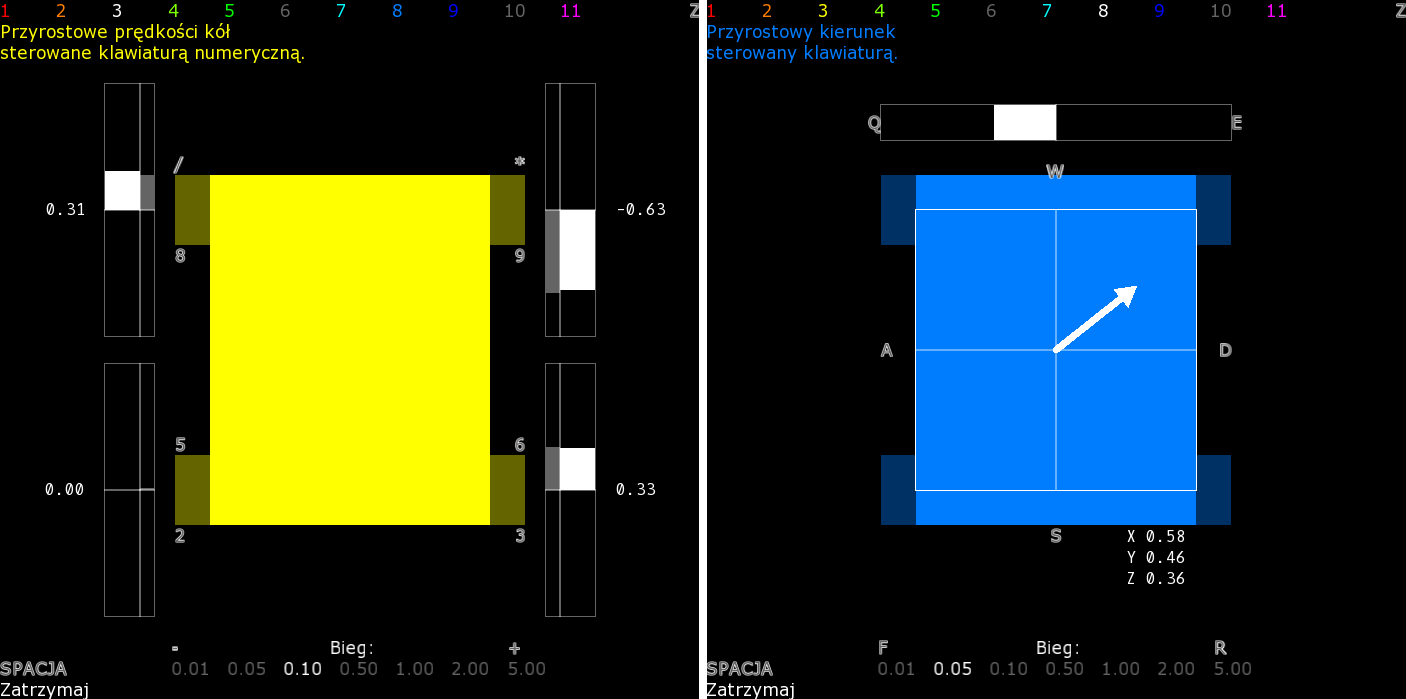
\includegraphics[width=0.8\textwidth]{graphics/lalkarz.png}
			\caption{Zrzuty ekranu dwóch trybów działania programu.}
			\label{fig:lalkarz}
			\end{figure}

			
		

